
% This LaTeX was auto-generated from MATLAB code.
% To make changes, update the MATLAB code and republish this document.

\documentclass{article}
\usepackage{graphicx}
\usepackage{color}

\sloppy
\definecolor{lightgray}{gray}{0.5}
\setlength{\parindent}{0pt}

\begin{document}

    
    
\section*{ECE300: Communication Theory HW 3}


\subsection*{Contents}

\begin{itemize}
\setlength{\itemsep}{-1ex}
   \item Question 7
   \item Question 8
\end{itemize}
\begin{par}
Initialization of variables
\end{par} \vspace{1em}
\begin{verbatim}
% Author: Daniel Kim
% Professor: Brian L. Frost
% 9/25/20
\end{verbatim}


\subsection*{Question 7}

\begin{verbatim}
clear; close all; clc
w=linspace(-pi*1000,pi*1000,10001);
variance = 1000;
M = 1000;
m = linspace(-1000,1000,2001);
noisevec = sqrt(variance)*randn(1,500000); % white noise
[rx, psd] = AutoCorrelation(noisevec,M);
\end{verbatim}
\begin{par}
Plot
\end{par} \vspace{1em}
\begin{verbatim}
figure;
subplot(2,1,1);
stem(m,rx);
xlabel('m');
title('Autocorrelation of White Noise')
subplot(2,1,2);
semilogy(w,abs(psd));
ylim([1,3000]);
xlabel('w');
title('PSD of White Noise');
\end{verbatim}

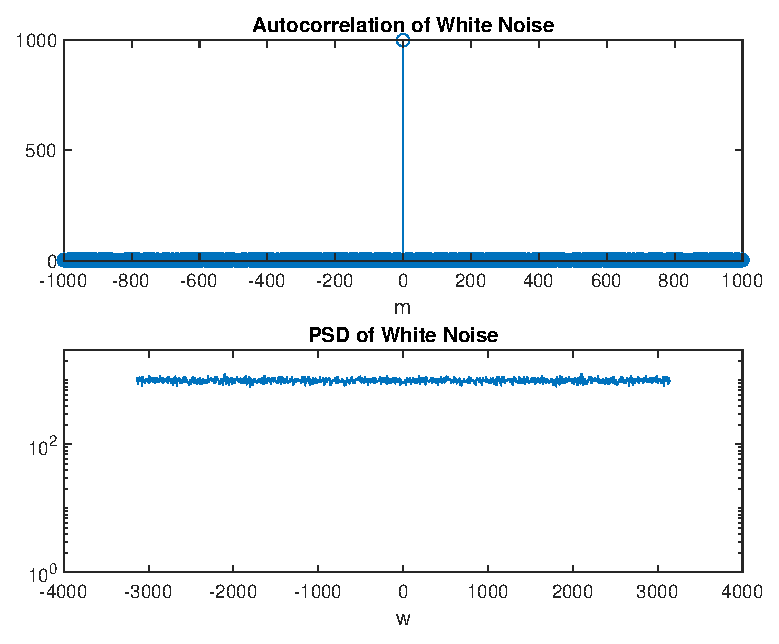
\includegraphics [width=4in]{ECE300_HW3_01.eps}
\begin{par}
The autocorrelation of white noise looks like a delta and the PSD looks like a flat line.
\end{par} \vspace{1em}


\subsection*{Question 8}

\begin{verbatim}
Y = sqrt(variance)*randn(1,500000);
Z = sqrt(variance)*randn(1,500000);
t = linspace(0,10,500000);
X = Y.*cos(10000*t) + Z.*sin(10000*t);
[x_rx,x_psd] = AutoCorrelation(X,M);
\end{verbatim}
\begin{par}
Plot
\end{par} \vspace{1em}
\begin{verbatim}
figure;
semilogy(w,abs(x_psd));
ylim([.001,3000]);
title('PSD of x(t)');
xlabel('w');
x_psd_integral = x_psd./(w.*w);
figure;
semilogy(w,abs(x_psd_integral));
title('PSD of integral of x(t)');
xlabel('w');
\end{verbatim}

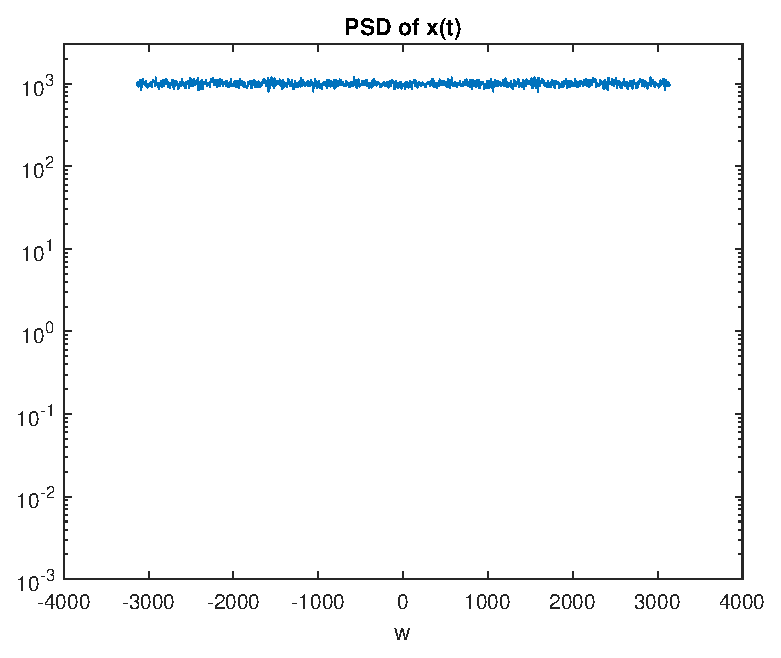
\includegraphics [width=4in]{ECE300_HW3_02.eps}

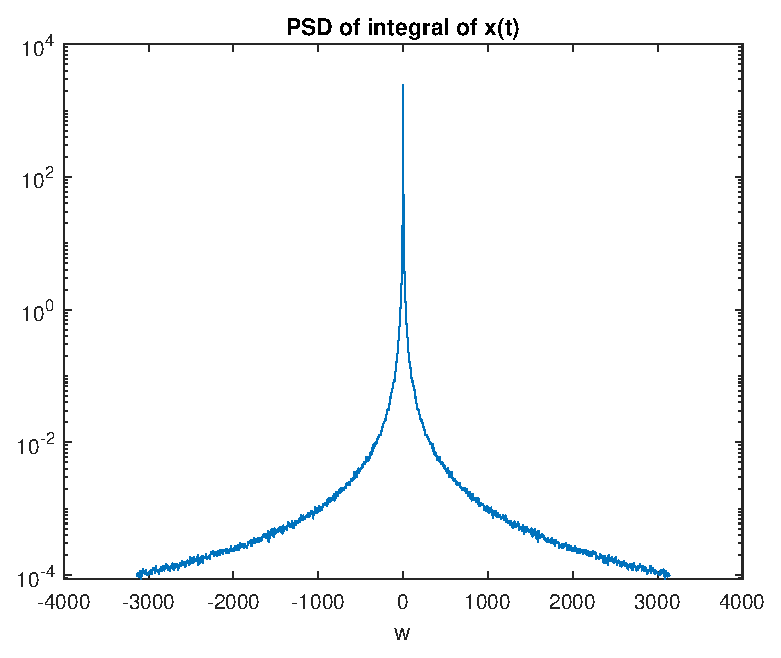
\includegraphics [width=4in]{ECE300_HW3_03.eps}



\end{document}

